% 规定文档类型
%\documentclass[12pt, a4paper, oneside,draft]{ctexart} % 草稿模式
\documentclass[12pt, a4paper, oneside]{ctexart} % 成品模式


% ------------导包区(我自创的名字)导入宏包,根据需要去删改----------------
\usepackage{amsmath, amsthm, amssymb, graphicx}
\usepackage[bookmarks=true, colorlinks, citecolor=blue, linkcolor=black]{hyperref}
\usepackage{listings}
\usepackage{xcolor} % 自定义颜色
\definecolor{str_color}{RGB}{118, 161, 79}
\definecolor{background_color}{RGB}{250,250,250}
\definecolor{key_color}{RGB}{166, 102, 194}
\definecolor{comment_color}{RGB}{0, 0, 255}
\usepackage{subcaption} % 多图
\usepackage{booktabs} % 表格粗框线
\usepackage{float} % 使用H替代htbp来精确控制图片/表格的位置
\usepackage{algorithm} % 伪代码自动加框线
\usepackage{algorithmic} % 伪代码语句
\usepackage{hyperref} %导入超链接
\usepackage{titlesec}

% ------------导言区,这里规定了标题等各种功能信息-------------
\title{深度学习实战-图像识别篇 \\ \large 预训练模型图像分类}
\author{POET}
\date{\today}
% 如果要使用页面操作,规定页面参数,就要用到geometry宏包
% 然后在导言区使用\geometry{left=2.54cm, right=2.54cm, top=3.18cm, bottom=3.18cm}
% 行间距也可以使用\linespread{1.5}来设置
% 页码也可以自定义\pagenumering{roman}

% 这里创造了很多定理环境,写中文定理,推论的时候可以用
\newtheorem{theorem}{定理}[section]
\newtheorem{definition}[theorem]{定义}  
\newtheorem{lemma}[theorem]{引理}
\newtheorem{corollary}[theorem]{推论}
\newtheorem{example}[theorem]{例}
\newtheorem{proposition}[theorem]{命题}

% 设置直接生成的代码风格
\lstset{
    % 格式控制
    language=Python,
    basicstyle=\small,% 设置基本字体
    numbers=left, %设置行号位置
    numberstyle=\tiny, %设置行号大小
    escapeinside=``, %逃逸字符(1左面的键),用于显示中文
    breaklines, %自动折行
    extendedchars=false, %解决代码跨页时,章节标题,页眉等汉字不显示的问题
    xleftmargin=2em,xrightmargin=2em, aboveskip=1em, %设置边距
    tabsize=4, %设置tab空格数
    showspaces=false, %不显示空格
    frame=single, %设置边框格式
    % 颜色控制,本人独爱dracula风格。
    % 只能用注释断行,但是还是容易出现各种玄学问题
    % basicstyle=\color{black},
    backgroundcolor=\color{background_color},
    keywordstyle=\color{key_color}, %设置关键字颜色
    stringstyle=\color{str_color}, % 设置字符串颜色
    commentstyle=\color{comment_color}, %设置注释颜色
}
% -------------正文区-----------------------

\begin{document}

\maketitle  % 这一句将上面导言区的设置实现出来

    % \begin{abstract}
    %     这是摘要这是摘要这是摘要这是摘要这是摘要这是摘要这是摘要这是摘要这是摘要
    %     这是摘要这是摘要这是摘要这是摘要这是摘要这是摘要这是摘要这是摘要这是摘要
    %     这是摘要这是摘要这是摘要这是摘要 \\[8pt] %调节间距
    %     \textbf{关键词:关键词1 \ 关键词2}
    % \end{abstract}

    % \tableofcontents %生成目录

\newpage

上一章我们从网络上爬取图片,制作了自己的图像数据集,
并按照七三的比例将其分为训练集和测试集。这一章,我们学习
使用预训练好的模型对图像中的物体进行分类。

\section{载入预训练图像分类模型}

在torchvision.model中定义了许多模型用于计算机视觉的任务中:

\begin{itemize}
    \item 图像分类
    \item 语义分割
    \item 目标检测
    \item 实例分割
    \item 人物关键点检测
    \item 视频分类
\end{itemize}

下面将给出部分预训练模型的例子:

\begin{lstlisting}[language=Python]
    import torchvision.models as models

    resnet18 = models.resnet18()
    alexnet = models.alexnet()
    vgg16 = models.vgg16()
    squeezenet = models.squeezenet1_0()
    densenet = models.densenet161()
    inception = models.inception_v3()
    googlenet = models.googlenet()
    shufflenet = models.shufflenet_v2_x1_0()
    mobilenet = models.mobilenet_v2()
    resnext50_32x4d = models.resnext50_32x4d()
    wide_resnet50_2 = models.wide_resnet50_2()
    mnasnet = models.mnasnet1_0()
\end{lstlisting}

当pretrained参数为true时,就导入了训练的模型。


\section{准备数据集}

这一章使用上一章抓取的图片进行训练,这个数据集只包括四种不同的猫。


\subsection{加载数据集}

加载数据集代码如下所示:

\begin{lstlisting}[language=Python]
    from torchvision import datasets, transforms

    # 在训练集上:扩充、归一化
    # 在验证集上:归一化
    data_transforms = {
        'train': transforms.Compose([
            transforms.RandomResizedCrop(224),
            transforms.RandomHorizontalFlip(),
            transforms.ToTensor(),
            transforms.Normalize([0.485, 0.456, 0.406], [0.229, 0.224, 0.225])
        ]),
        'val': transforms.Compose([
            transforms.Resize(256),
            transforms.CenterCrop(224),
            transforms.ToTensor(),
            transforms.Normalize([0.485, 0.456, 0.406], [0.229, 0.224, 0.225])
        ]),
    }
    #数据集存放路径
    data_dir = 'data/hymenoptera_data'
    #使用torchvision.datasets.ImageFolder类快速封装数据集
    #此处使用了lambda语法
    image_datasets = {x: datasets.ImageFolder(os.path.join(data_dir, x),data_transforms[x])
                        for x in ['train', 'val']}
    dataloaders = {x: torch.utils.data.DataLoader(image_datasets[x], batch_size=4,shuffle=True, num_workers=4)
                    for x in ['train', 'val']}
    #读取数据集的数目
    dataset_sizes = {x: len(image_datasets[x]) for x in ['train', 'val']}
    #读取数据集中的图像种类
    class_names = image_datasets['train'].classes
\end{lstlisting}


\subsection{使用matplotliob可视化数据集}

由于一个batch中的图像是保存在tensor中,
一张维度是[H,W,C]、值范围是[0,255]的图片需要经过ToTensor转换成维度是[C,H,W]、
值范围是[0,1]的Tensor,在经过Normalize完成归一化。
而使用matplotlib显示的图像需要对图像进行反向操作才能正常显示。

\begin{lstlisting}
    import matplotlib.pyplot as plt

    def imshow(inp, title=None): 
        # 可视化一组 Tensor 的图片
        inp = inp.numpy().transpose((1, 2, 0)) #转换图片维度
        mean = np.array([0.485, 0.456, 0.406]) 
        std = np.array([0.229, 0.224, 0.225]) 
        inp = std * inp + mean #反向操作
        inp = np.clip(inp, 0, 1) 
        plt.imshow(inp) 
        if title is not None: 
            plt.title(title) 
        plt.pause(0.001) # 暂停一会儿,为了将图片显示出来
    # 获取一批训练数据
    inputs, classes = next(iter(dataloaders['train'])) 
    # 批量制作网格
    out = torchvision.utils.make_grid(inputs) 
    imshow(out, title=[class_names[x] for x in classes]) 
\end{lstlisting}

运行结果如下图所示:

\begin{figure}[H]
    \centering
    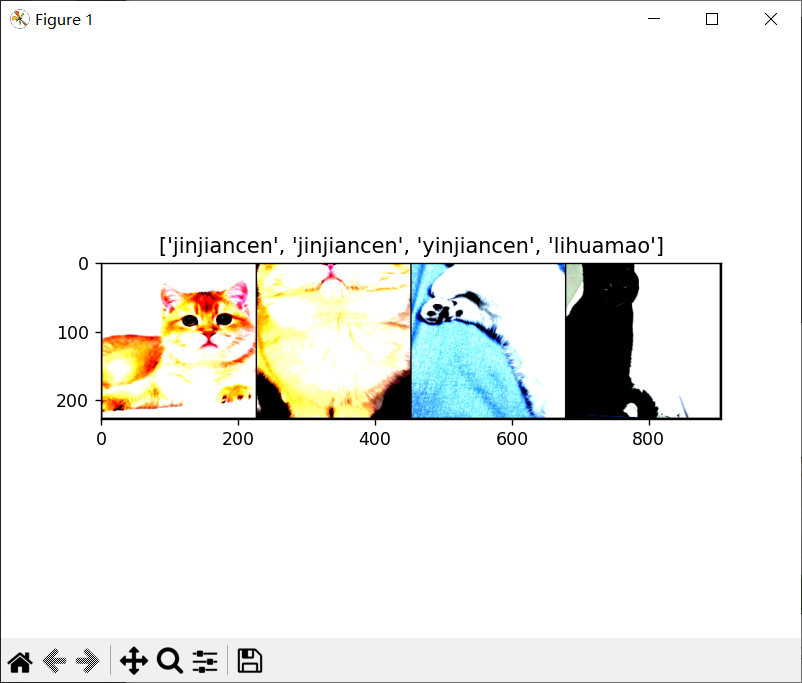
\includegraphics[width=0.9\textwidth]{1.png}
\end{figure}


\section{模型训练函数}

虽然ResNet模型有训练好的参数,但是我们还是要进行训练。
下面的代码进行了五次训练,并展示出每个epoch的准确度。
这个函数包括加载模型,正向传播,计算损失函数,利用优化器进行学习优化的过程。

\begin{lstlisting}
    def train_model(model, criterion, optimizer, scheduler, num_epochs=25): 
    """ 训练模型,并返回在验证集上的最佳模型和准确率 
    Args: 
    - model(nn.Module): 要训练的模型 
    - criterion: 损失函数 
    - optimizer(optim.Optimizer): 优化器 
    - scheduler: 学习率调度器 
    - num_epochs(int): 最大 epoch 数 
    Return: 
    - model(nn.Module): 最佳模型 
    - best_acc(float): 最佳准确率 
    """
    since = time.time()

    best_model_wts = copy.deepcopy(model.state_dict())
    best_acc = 0.0

    for epoch in range(num_epochs):
        print(f'Epoch {epoch}/{num_epochs - 1}')
        print('-' * 10)

        # 训练集和验证集交替进行前向传播
        for phase in ['train', 'val']:
            if phase == 'train':
                model.train()  # 设置为训练模式,可以更新网络参数
            else:
                model.eval()   # 设置为预估模式,不可更新网络参数

            running_loss = 0.0
            running_corrects = 0

            # 遍历数据集
            for inputs, labels in dataloaders[phase]:
                inputs = inputs.to(device)
                labels = labels.to(device)

                # 清空梯度,避免累加了上一次的梯度
                optimizer.zero_grad()

                with torch.set_grad_enabled(phase == 'train'):
                    # 正向传播
                    outputs = model(inputs)
                    _, preds = torch.max(outputs, 1)
                    loss = criterion(outputs, labels)

                    # 反向传播且仅在训练阶段进行优化
                    if phase == 'train':
                        loss.backward() # 反向传播
                        optimizer.step()

                # 统计loss、准确率
                running_loss += loss.item() * inputs.size(0)
                running_corrects += torch.sum(preds == labels.data)
            if phase == 'train':
                scheduler.step()

            epoch_loss = running_loss / dataset_sizes[phase]
            epoch_acc = running_corrects.double() / dataset_sizes[phase]

            print(f'{phase} Loss: {epoch_loss:.4f} Acc: {epoch_acc:.4f}')

            # 发现了更优的模型,记录起来
            if phase == 'val' and epoch_acc > best_acc:
                best_acc = epoch_acc
                best_model_wts = copy.deepcopy(model.state_dict())

        print()

    time_elapsed = time.time() - since
    print(f'Training complete in {time_elapsed // 60:.0f}m {time_elapsed % 60:.0f}s')
    print(f'Best val Acc: {best_acc:4f}')

    # 加载训练的最好的模型
    model.load_state_dict(best_model_wts)
    return model
\end{lstlisting}


\section{使用torchvision微调模型}

因为ResNet模型的全连接层输出为1000层,而我们的数据集输出应该仅为4层,
所以要修改模型的fc,也就是全连接层,代码如下:

\subsection{不固定模型参数进行训练}

\textbf{注意,这种方法意味着使模型每一步都基于预训练的参数进行更新,一般我们需要将除了修改的输出层之外的层进行冻结,不更新参数,只基于前面层数提取出的特征进行训练。}

\begin{lstlisting}
    model = models.resnet18(pretrained=True) # 加载预训练模型
    num_ftrs = model.fc.in_features # 获取低级特征维度 
    model.fc = nn.Linear(num_ftrs, 2) # 替换新的输出层 
    model = model.to(device) 
    # 交叉熵作为损失函数 
    criterion = nn.CrossEntropyLoss() 
    # 所有参数都参加训练 
    optimizer_ft = optim.SGD(model.parameters(), lr=0.001, momentum=0.9) 
    # 每过 7 个 epoch 将学习率变为原来的 0.1 
    scheduler = optim.lr_scheduler.StepLR(optimizer_ft, step_size=7, gamma=0.1)
    model_conv = train_model(model_conv, criterion, optimizer_conv, exp_lr_scheduler, num_epochs=5)
\end{lstlisting}


\subsection{固定模型参数}

微调预训练模型,需要修改模型的内部结构,使其符合具体任务。模型所用框架不一样,在 将其他框架编写的模型迁移到 PyTorch 中时,无法使它们兼容。此时可以采取 Pipeline 形式将预训 练模型的参数固定,或者说将前一个模型的输出保存下来,将该输出作为 PyTorch 模型的输入。


采取这种思路,我们可以将模型除了输出层之外的所有层看成一个特征提取器。在训练模型时,这些层的权重不参与训练,不可优化。在 PyTorch 中将权重设置为不可训练,只需将 requires-grad 设置为 False 即可。例如,下述代码可以将 ResNet18 的所有层设置为不可训练。

\begin{lstlisting}
    model_conv = torchvision.models.resnet18(pretrained=True) # 加载预训练模型
    for param in model_conv.parameters(): # 锁定模型所有参数
        param.requires_grad = False
    
    num_ftrs = model_conv.fc.in_features  # 获取低级特征维度
    model_conv.fc = nn.Linear(num_ftrs, 2) # 替换新的输出层
    
    model_conv = model_conv.to(device)
    
    criterion = nn.CrossEntropyLoss()
    
    # 只有最后一层全连接层fc,参加训练
    optimizer_conv = optim.SGD(model_conv.fc.parameters(), lr=0.001, momentum=0.9)
    
    # 每过 7 个 epoch 将学习率变为原来的 0.1 
    exp_lr_scheduler = lr_scheduler.StepLR(optimizer_conv, step_size=7, gamma=0.1)
    model_conv = train_model(model_conv, criterion, optimizer_conv,
                             exp_lr_scheduler, num_epochs=5)
    visualize_model(model_conv)
    
    plt.ioff()
    plt.show()
    
\end{lstlisting}

结果如下图:

\begin{figure}[H]
\centering
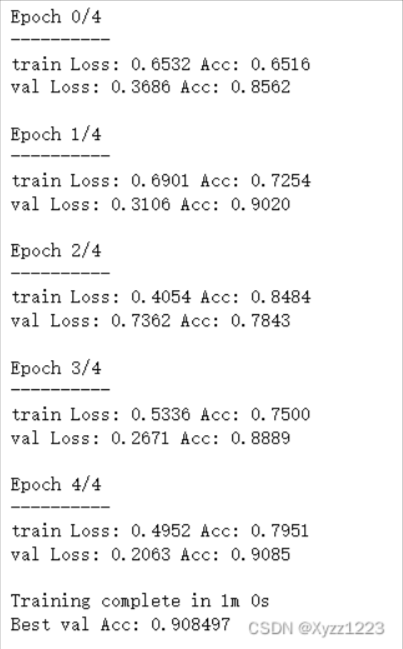
\includegraphics[width=0.5\textwidth]{2.png}
\end{figure}


\section{观察模型预测结果}

接下来将模型切换到eval模式,也就是对测试集进行预测,并可视化结果:

\begin{lstlisting}
    def visualize_model(model, num_images=6):
    was_training = model.training
    model.eval()
    images_so_far = 0
    fig = plt.figure()

    with torch.no_grad():
        for i, (inputs, labels) in enumerate(dataloaders['val']):
            inputs = inputs.to(device)
            labels = labels.to(device)

            outputs = model(inputs)
            _, preds = torch.max(outputs, 1)

            for j in range(inputs.size()[0]):
                images_so_far += 1
                ax = plt.subplot(num_images//2, 2, images_so_far)
                ax.axis('off')
                ax.set_title(f'predicted: {class_names[preds[j]]}')
                imshow(inputs.cpu().data[j])

                if images_so_far == num_images:
                    model.train(mode=was_training)
                    return
        model.train(mode=was_training)
visualize_model(model_conv)

plt.ioff()
plt.show()
\end{lstlisting}

预测结果如下图:

\begin{figure}[H]
    \centering
    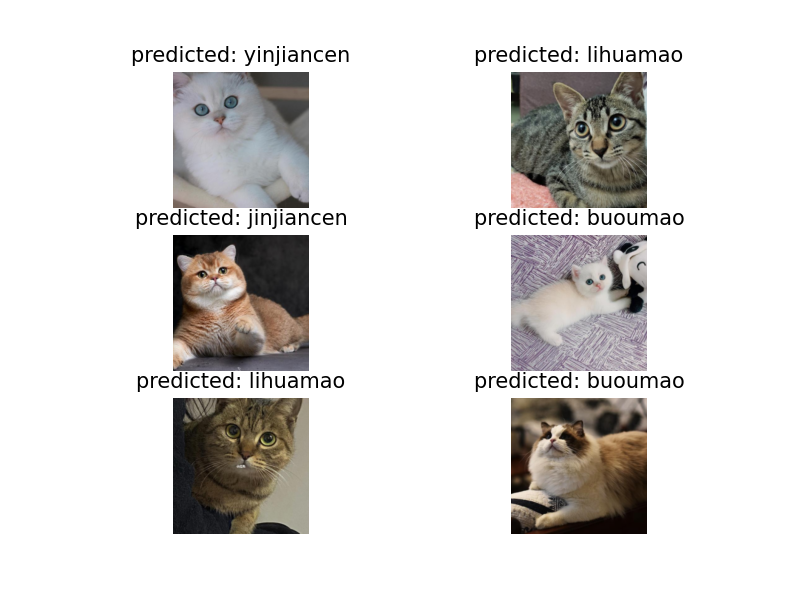
\includegraphics[width=1\textwidth]{3.png}
\end{figure}

可以看出预测准确度很高。
\end{document}